\documentclass[tikz, border=1mm]{standalone}
\usepackage{tikz}
\usetikzlibrary{backgrounds}
\usepackage{xcolor,calc}

\begin{document}


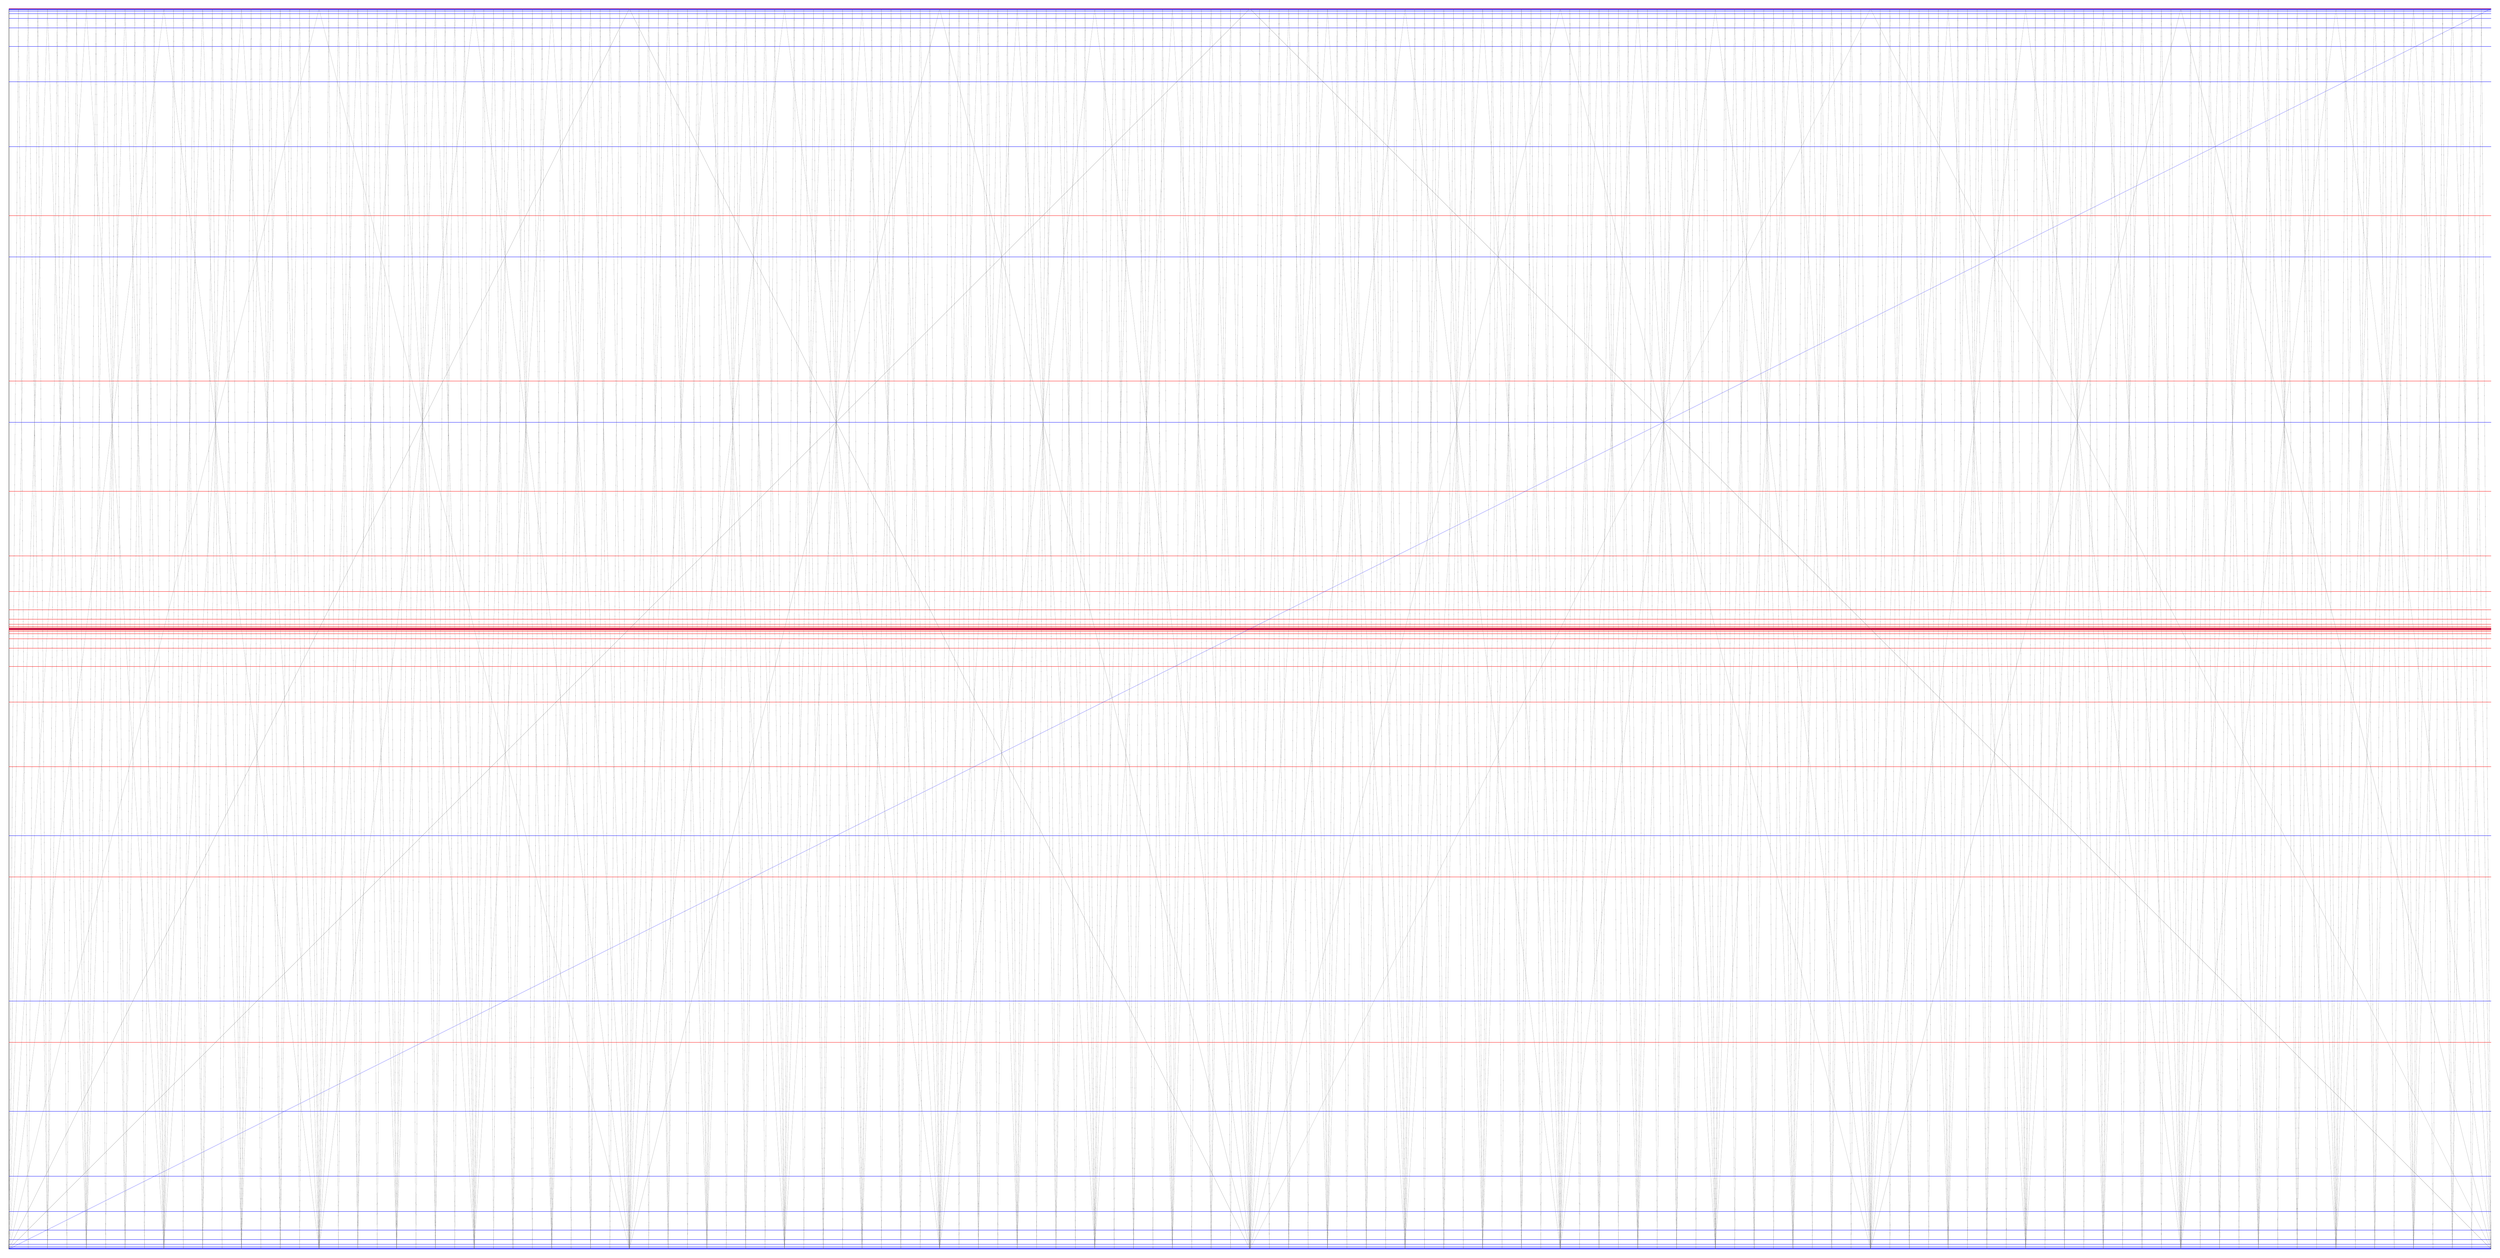
\begin{tikzpicture}[
    scale=50,
    background rectangle/.style={fill=white},
    show background rectangle
]
    % Define rectangle dimensions
    \def\rectheight{1};
    \def\rectwidth{2*\rectheight};
        \clip (0,0) rectangle (\rectwidth,\rectheight);
    
    % Draw the original rectangle
    \draw[ultra thin] (0,0) rectangle (\rectwidth,\rectheight);
    
            \foreach \k in {0,...,12} {
                                        \pgfmathsetmacro{\mythickness}{0.1}%{0.001*(1-\n*0.005)}%{0.1-0.05*\n}
                                        \pgfmathsetmacro{\magicheightup}{2^\k/(2^\k+1)*\rectheight}
                                \pgfmathsetmacro{\magicheightdown}{1/(2^\k+1)*\rectheight}
                \draw[color=blue,line width=\mythickness pt] (0,\magicheightup) -- (\rectwidth,\magicheightup) ;
                        \draw[color=blue,line width=\mythickness pt] (0,\magicheightdown) -- (\rectwidth,\magicheightdown) ;
                        
                        
                            \pgfmathsetmacro{\magicheighttop}{\rectheight*(1/2+1/(2^\k+1))}
                                \pgfmathsetmacro{\magicheightbottom}{\rectheight*(1/2-1/(2^\k+1)}
                                \draw[color=red,line width=0.1pt] (0,\magicheighttop) -- (\rectwidth,\magicheighttop);
                   \draw[color=red,line width=0.1pt] (0,\magicheightbottom) -- (\rectwidth,\magicheightbottom);
                   }
    % Draw the diagonals with increasing colors from blue to red
    \draw[ultra thin, blue] (0,0) -- (\rectwidth,\rectheight);
        \foreach \n in {7,...,0} {
        \pgfmathsetmacro{\numtriangles}{2^\n-1}\\
        \foreach \m in {\numtriangles,...,0} {
                    \pgfmathsetmacro{\startx}{\m*\rectwidth/2^\n}
            \pgfmathsetmacro{\endx}{(\m+1)*\rectwidth/2^\n}
              \pgfmathsetmacro{\myopacity}{60}%{100-\n*pi}
                            \pgfmathsetmacro{\mythickness}{0.1}%{0.001*(1-\n*0.005)}%{0.1-0.05*\n}

                            \definecolor{mycolor}{RGB}{0, 0, 0}

                               

            \draw[color=mycolor!\myopacity, line width=0.1pt] (\startx,0) -- ({\startx+(\endx-\startx)/2},\rectheight);
            \draw[color=mycolor!\myopacity, line width=0.1pt] ({\startx+(\endx-\startx)/2},\rectheight) -- (\endx,0);
            


}
    }
    
    % Add a note about scaling
    \node[below] at (\rectwidth/2,-0.5) {Note: horizontal distances shown at decreasing scale for clarity};
\end{tikzpicture}

\end{document}